%%%%%%
%
% $Autor: Sudeshna Nanda $
% $Date: 2025-01-15 $
% $File name:  ProjectPresentation.tex
% $Version: 1.0 $
%
% !TeX encoding = utf8
%
%%%%%%

\Mysection{Introduction}

\begin{frame}{Introduction}
	\begin{itemize}
		\item \textbf{The Synergy of Machine Learning and IoT}
		\begin{itemize}
			\item IoT has revolutionized industries like healthcare, agriculture, and smart cities \cite{Had:2020}.
			\item Many IoT applications demand real-time data processing, unsuitable for traditional cloud computing \cite{Shi:2016}.
		\end{itemize}
		
		\item \textbf{Emergence of TinyML}
		\begin{itemize}
			\item Enables low-latency, low-power, and efficient model inference on edge devices \cite{Sakr:2020}.
			\item Operates on compact devices (e.g., RTOS-based microcontrollers) with long battery life \cite{Anh:2009} \cite{Aba:2023}.
		\end{itemize}
	\end{itemize}
\end{frame}
\begin{frame}{Introduction}
	\begin{itemize}
		\item \textbf{Arduino and Its Evolution}
		\begin{itemize}
			\item Initially a prototyping tool, now supports IoT, wearables, and embedded systems \cite{Kushner:2011}.
			\item Arduino Nano 33 BLE Sense: A 3.3V board featuring embedded sensors like accelerometers for motion detection \cite{Ard:2021}.
		\end{itemize}
		\item \textbf{Objective of the Study}
		\begin{itemize}
			\item Develop a \textbf{"Magic Wand"} using Arduino Nano 33 BLE Sense.
			\item Program the board to recognize predefined gestures (e.g., wing, ring, slope).
		\end{itemize}
	\end{itemize}
\end{frame}


\begin{frame}{Project Overview}
	\begin{block}{\textbf{Hardware: Arduino Nano 33 BLE Sense}}
		\begin{itemize}
			\item \textbf{Embedded Sensors:} Three-axis accelerometer for precise motion detection \cite{Arduino, 2021}.
			\item \textbf{Compact and Energy-efficient Design:} Ideal for portable and edge-based applications.
			\item \textbf{Integration with ML Frameworks:} Supports TensorFlow Lite for deploying optimized models.
		\end{itemize}
	\end{block}
	
	\begin{block}{\textbf{Project Objective}}
		\begin{itemize}
			\item Develop a \textbf{Magic Wand} for real-time gesture recognition.
			\item Recognize predefined gestures such as wing, ring, and slope.
			\item Integrate lightweight ML models with Arduino Nano 33 BLE Sense for efficient, low-latency inference.
		\end{itemize}
	\end{block}
\end{frame}
\begin{frame}{Project Overview}
	\begin{block}{\textbf{Output}}
		\begin{itemize}
		
			\item \textbf{Screen Visualization:} Displays real-time gesture recognition results on a terminal.
		\end{itemize}
	\end{block}
	
	\begin{block}{\textbf{Enhanced Execution and Future Enhancements}}
		\begin{itemize}
			\item \textbf{Gesture Precision:} Optimized ML models to minimize false readings and ensure accuracy.
			\item \textbf{Edge Intelligence:} Leverage TinyML for efficient and low-latency performance on edge devices.
			\item \textbf{Future Enhancements:}
			\begin{itemize}
				\item Expand gesture recognition capabilities.
				\item Further optimize performance and power efficiency.
					
			\end{itemize}
		\end{itemize}
	\end{block}
\end{frame}


\section{Model Implementation}
\begin{frame} \frametitle{Model Implementation and Futuristic Functions}
	
	\begin{block}{\textbf{TensorFlow Lite (TFLite)}}
		\begin{itemize}
			\item Framework for deploying machine learning models on resource-constrained devices.
			\item Facilitates model optimization using techniques which are quantization and pruning.
			\item Enables real-time gesture recognition through efficient edge inference.
		\end{itemize}
	\end{block}
	
	\begin{block}{\textbf{TensorFlow Lite Micro (TFLite Micro)}}
		\begin{itemize}
			\item Tailored for microcontrollers, including Arduino Nano 33 BLE Sense.
			\item Executes quantized models within the device's memory and computational limitations.
			\item Seamless integration with existing Arduino libraries for gesture-based applications.
		\end{itemize}
	\end{block}
\end{frame}
\begin{frame}
	\begin{block}{\textbf{Model Training Process}}
		\begin{itemize}
			\item \textbf{Data Collection:} Gather accelerometer data for gestures like "wing," "ring," and "slope."
			\item \textbf{Preprocessing:} Normalize and augment data to enhance model performance.
			\item \textbf{Training and Optimization:} 
			\begin{itemize}
				\item Utilize CNNs for feature extraction and classification.
				\item Apply quantization and pruning to reduce memory footprint.
			\end{itemize}
		\end{itemize}
	\end{block}
	
	\begin{block}{\textbf{Futuristic Enhancements}}
		\begin{itemize}
			\item Use Remotexy to operate the Magic Wand for its dynamic movements.
			\item Enchance the model by showing digital output on Arduino using Pico4ML and Pico2.
			\item Explore advanced optimization techniques, such as knowledge distillation, to enhance efficiency.
		\end{itemize}
	\end{block}
\end{frame}

\section{Gesture Types}
\begin{frame}{Gesture Types}
	Dataset Collection and labeling of data for three trained movements: wing (W), ring (O), and slope (/).The following figures show the direction of motion and shape for each gesture. [\cite{War:2020}]
	\begin{figure}[H]\centering
		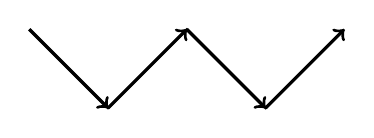
\begin{tikzpicture}
			% define point
			\coordinate (A)  at (1, 1);
			\coordinate (O)  at (2, 0);
			\coordinate (B)  at (3, 1);
			\coordinate (C)  at  (4,0);
			\coordinate (D) at  (5,1);
			% angle  
			\draw[thick] (A) -- (O) -- (B) -- (C)-- (D);
			%	\draw pic[draw=black,eccentricity=2.9]
			%\pic [draw,"$\alpha_1$",angle radius=20,->,angle eccentricity=1.4]
			%  {angle = B--O--A};
			\draw [->, very thick] (1,1) -- (2,0)  node [midway, above] {\scriptsize };
			\draw [->, very thick] (2,0) -- (3,1)  node [midway, above] {\scriptsize };
			\draw [->, very thick] (3,1) -- (4,0)  node [midway, above] {\scriptsize };
			\draw [->, very thick] (4,0) -- (5,1)  node [midway, above] {\scriptsize };
		\end{tikzpicture}
		{\textbf{Wing Gesture }}
		\label{fig:Wing Gesture}
	\end{figure}
	
	\begin{figure}[H]\centering
		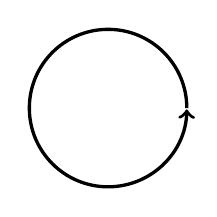
\begin{tikzpicture}
			\draw[->,very thick] (0,0) arc[radius=1cm,start angle=0,delta angle=359];
		\end{tikzpicture}
		{\textbf{Ring Gesture }}
		\label{fig:Ring Gesture}
	\end{figure}
	
	\begin{figure}[H]\centering
		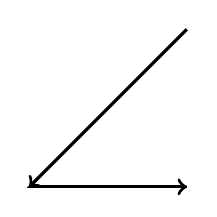
\begin{tikzpicture}
			% define point
			\coordinate (A)  at (2, 2);
			\coordinate (O)  at (0, 0);
			\coordinate (B)  at (2, 0);
			% angle  
			\draw[thick] (A) -- (O) -- (B);
			%\draw pic[draw=black,angle radius=20,angle eccentricity=1.4]
			%{angle = B--O--A};
			%\pic [draw,"$\alpha_1$",angle radius=20,->,angle eccentricity=1.4]
			%  {angle = B--O--A};
			\draw [->, very thick] (2,2) -- (0,0)  node [midway, above] {\scriptsize };
			\draw [->, very thick] (0,0) -- (2,0)  node [midway, above] {\scriptsize };
		\end{tikzpicture}
		{\textbf{Slope Gesture }}
		\label{fig:Slope Gesture}
	\end{figure}
	
\end{frame}

